\documentclass[conference]{IEEEtran}
\IEEEoverridecommandlockouts
\usepackage{matlab-prettifier}
\usepackage{cite}
\usepackage{amsmath,amssymb,amsfonts}
\usepackage{algorithmic}
\usepackage{graphicx}
\usepackage{textcomp}
\usepackage{xcolor}
\usepackage{float}
\def\BibTeX{{\rm B\kern-.05em{\sc i\kern-.025em b}\kern-.08em
    T\kern-.1667em\lower.7ex\hbox{E}\kern-.125emX}}

\begin{document}

\title{Project 3 : Importance Sampling}

\author{\IEEEauthorblockN{Owen Sowatzke}
\IEEEauthorblockA{\textit{Electrical Engineering Department} \\
\textit{University of Arizona}\\
Tucson, USA \\
osowatzke@arizona.edu}}
\maketitle

\begin{abstract}
Importance Sampling (IS) is an alternative to Monte Carlo (MC) simulation that can be used to estimate probabilities of hard-to-sample distributions. It more frequently samples the "important" samples of a distribution to reduce the variance of probability estimates. This document compares probabilities estimated with Monte Carlo Simulation and Importance Sampling. It specifically examines a case in which Monte Carlo Sampling provides very few "important" samples.
\end{abstract}

\begin{IEEEkeywords}
Monte Carlo Simulation, Importance Sampling,  Variance, Probability Estimates
\end{IEEEkeywords}

\section{Introduction}
Both Monte Carlo (MC) Simulations and Importance Sampling (IS) are techniques for estimating probabilities. In this document, both techniques will be used to estimate the probability that a random variable $X$ with distribution $X\sim N(1,1)$ exceeds 3.957 (i.e. $P\{X > 3.957\}$).
\section{Monte Carlo Simulation}
The probability of interest can be written as follows:
\begin{equation}
P\{X > 3.957\} = \int_{-\infty}^{\infty}I(x)f_X(x)dx
\label{Pint}
\end{equation}
where
\begin{equation}
I(x) = \begin{cases}
1 & x > 3.957 \\
0 & x \leq 3.957
\end{cases}
\label{Ix_def}
\end{equation}
Note that this probability can also be written as an expected value:
\begin{equation}
P\{X > 3.957\} = E[I(X)]
\end{equation}
Monte Carlo Simulation attempts to estimate this probability using a sample mean
\begin{equation}
P\{X > 3.957\} \approx \frac{1}{N}\sum_{i=1}^{N}I(x_i)
\end{equation}
where
\begin{equation}
x_1, x_2, ..., x_N \sim f_X(x)
\end{equation}
\par
Given different values of $N \in [1, 10^5]$, Monte Carlo Simulations can be used to estimate $P\{X > 3.957\}$. This estimate can than be compared to the true probability.
\begin{equation}
P\{X > 3.957\} = 0.001553
\end{equation}
The Monte Carlo probability estimate was generated for values $N$ from $100$ to $10^5$ in increments of $100$. The MATLAB code to generate this estimate is included in Appendix \ref{matlab_code}. The Monte Carlo probability estimate is plotted vs $N$ in Fig. \ref{Monte Carlo Estimate}
\begin{figure}[H]
\centerline{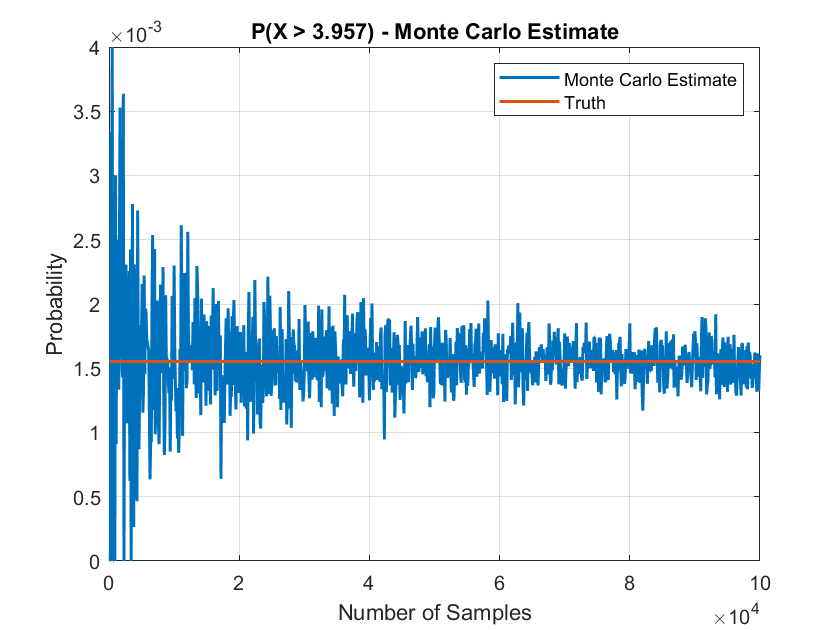
\includegraphics[width=0.5\textwidth]{Monte_Carlo_Estimate.png}}
\caption{Monte Carlo Probability Estimate}
\label{Monte Carlo Estimate}
\end{figure}
\noindent
The absolute value of the error between the Monte Carlo estimate and the true probability ($|P_{est}\{X > 3.957\} - P_{truth}\{X > 3.957\}|$) is also plotted vs $N$.
\begin{figure}[H]
\centerline{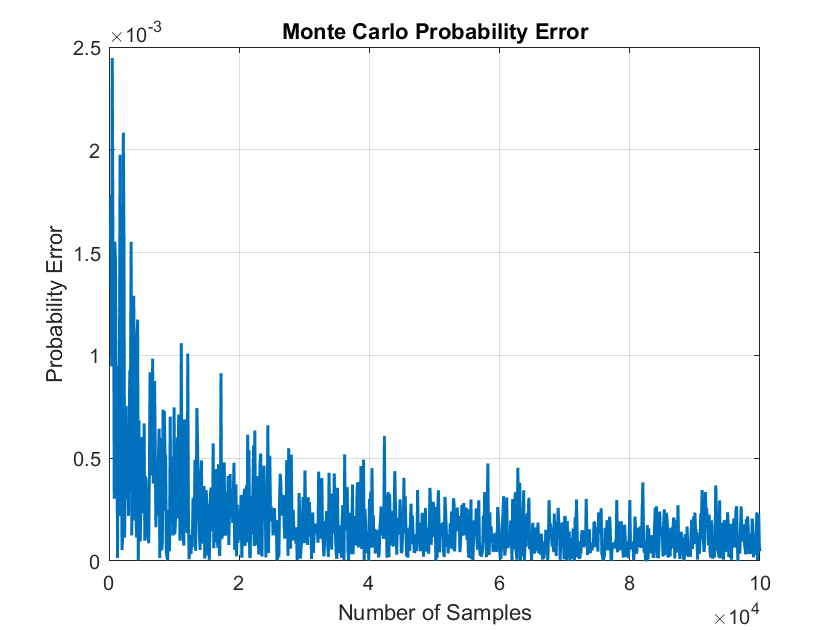
\includegraphics[width=0.5\textwidth]{Monte_Carlo_Error.png}}
\caption{Monte Carlo Probability Error}
\label{Monte Carlo Perr}
\end{figure}
As $N\rightarrow\infty$, the Monte Carlo Estimate should approach the true probability. This is confirmed by examining the results shown in Fig. \ref{Monte Carlo Perr}.
\section{Importance Sampling}
Examining the shaded area shown in Fig. 
\ref{Monte Carlo Limits}, very few of the samples from $f_X(x)$ contribute to the Monte Carlo probability estimate. This leads to large variances in the estimated probability.
\begin{figure}[H]
\centerline{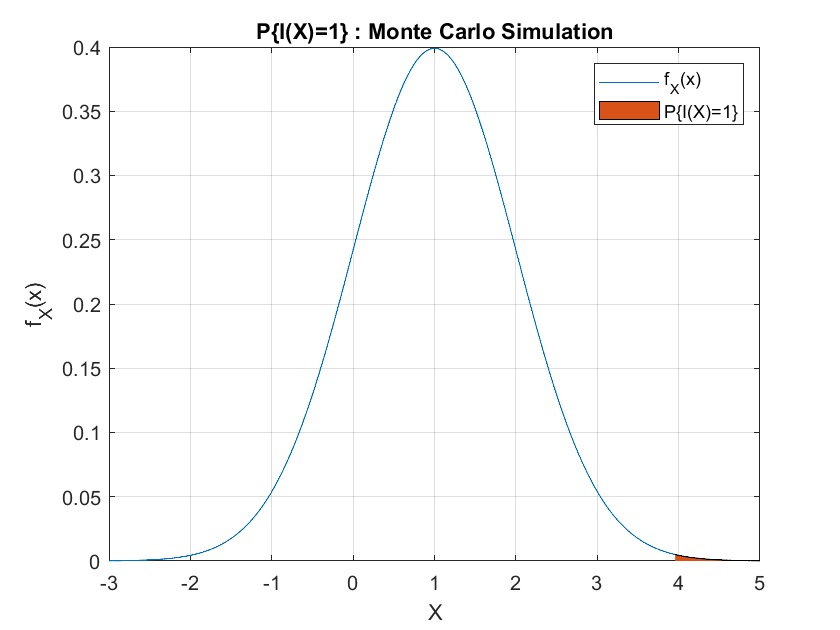
\includegraphics[width=0.5\textwidth]{MC_Indicator.png}}
\caption{Important Samples from $f_X(x)$}
\label{Monte Carlo Limits}
\end{figure}
Importance Sampling attempts to overcome these limitations. It re-expresses equation \eqref{Pint} in the following form:
\begin{equation}
P\{X > 3.957\} = \int_{-\infty}^{\infty}I(x)f_X(x)\frac{g_X(x)}{g_X(x)}dx
\label{is_int}
\end{equation}
where $I(x)$ is given by equation \eqref{Ix_def}.
Equation \eqref{is_int} can be also be written as follows:
\begin{equation}
P\{X > 3.957\} = \int_{-\infty}^{\infty}\left[I(x)\frac{f_X(x)}{g_X(x)}\right]g_X(x)dx
\end{equation}
This equation also represents an expected value.
\begin{equation}
P\{X > 3.957\} = E\left[I(x)\frac{f_X(x)}{g_X(x)}\right]
\end{equation}
Once again, the expected value can be estimated using a sample mean.
\begin{equation}
P\{X > 3.957\} \approx \frac{1}{N}\sum_{i=1}^{N}I(x_i)\frac{f_X(x_i)}{g_X(x_i)}
\label{is_prob_est}
\end{equation}
Note the samples $x_1,x_2,...,x_N$ are now sampled from $g_X(x)$ instead of $f_X(x)$. As such, the density function $g_X(x)$ can be selected to provide more "important" samples. 
\par
Consider a density $g_X(x)$ that is a shifted version of $f_X(x)$. Specifically, consider the following density function
\begin{equation}
g_X(x) = \frac{1}{\sqrt{2\pi}}e^{-(x-3.957)^2/2}
\end{equation}
The "important" samples of the new density function $g_X(x)$ are highlighted in Fig. \ref{Important Samples}. 
\begin{figure}[H]
\centerline{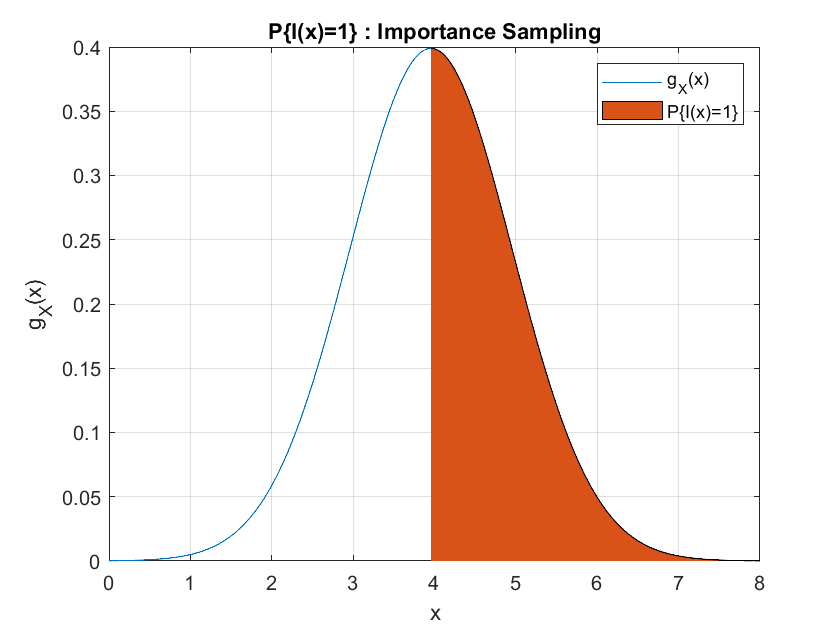
\includegraphics[width=0.5\textwidth]{IS_Indicator.png}}
\caption{Important Samples from $g_X(x)$}
\label{Important Samples}
\end{figure}
\noindent
Note that the number of important samples is significantly larger than that of Fig. \ref{Monte Carlo Limits}. This should reduce the variance of the probability estimate. 
\par
To confirm this result, an Importance Sampling probability estimate was generated for different values of $N$ using equation \eqref{is_prob_est}. The MATLAB code to generate this estimate is included in Appendix \ref{matlab_code}. The Important Sampling probability estimate is plotted vs $N$ in Fig. \ref{Importance Sampling Estimate}.
\begin{figure}[H]
\centerline{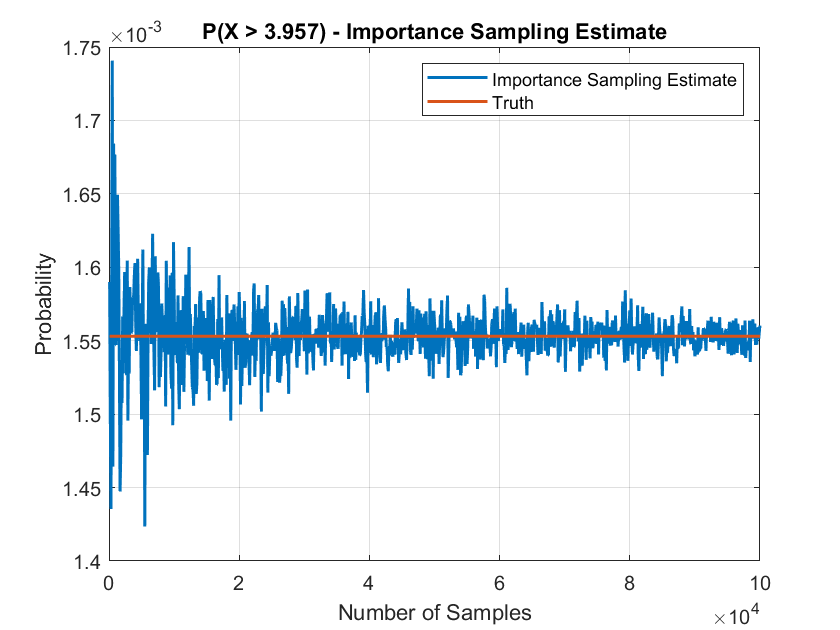
\includegraphics[width=0.5\textwidth]{Importance_Sampling_Estimate.png}}
\caption{Importance Sampling Probability Estimate}
\label{Importance Sampling Estimate}
\end{figure}
\noindent
The absolute value of the error between the Importance Sampling probability estimate and the true probability ($|P_{est}\{X > 3.957\} - P_{truth}\{X > 3.957\}|$) is also plotted vs $N$.
\begin{figure}[H]
\centerline{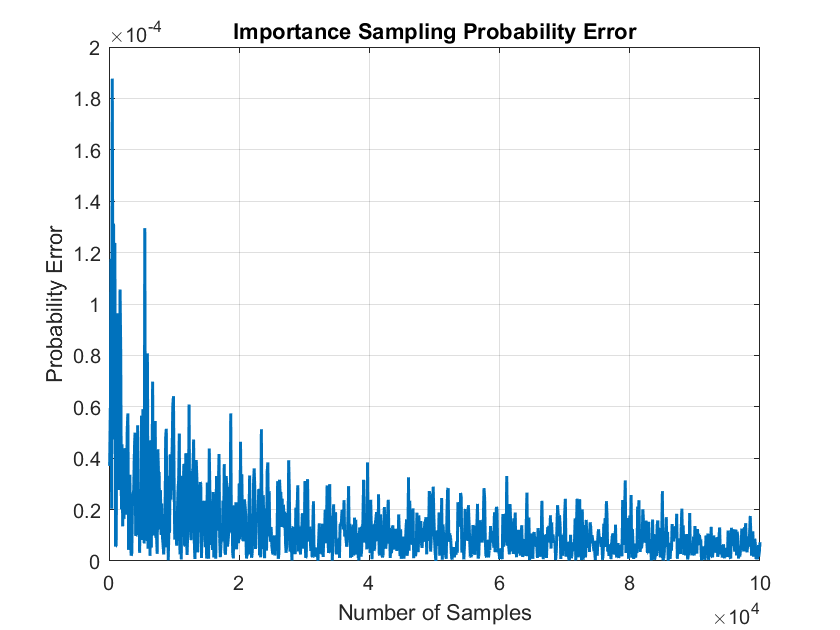
\includegraphics[width=0.5\textwidth]{Importance_Sampling_Error.png}}
\caption{Importance Sampling Probability Error}
\label{Importance Sampling Perr}
\end{figure}
The variance of the Monte Carlo and Importance Sampling probability estimates can be compared by overlaying the probability error plots. This plot is shown in Fig. \ref{Error Overlay}
\begin{figure}[H]
\centerline{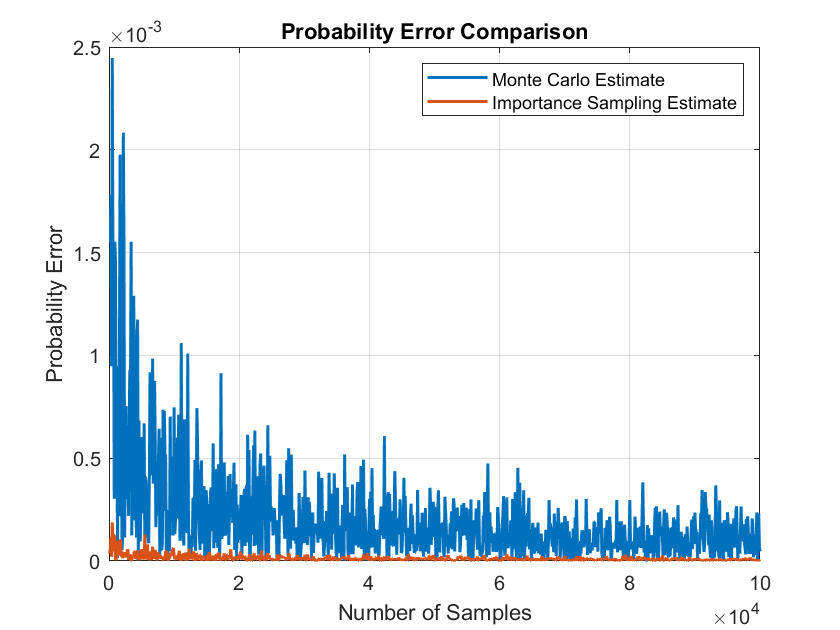
\includegraphics[width=0.5\textwidth]{Error_Overlay.png}}
\caption{Probability of Error Comparison}
\label{Error Overlay}
\end{figure}
\noindent
Note that the Importance Sampling probability estimate is much closer to the expected probability than the Monte Carlo Estimate. As such, the Importance Sampling estimate has a lower variance than the Monte Carlo Estimate for the same values of $N$.
\section{Conclusion}
Monte Carlo Simulation and Importance Sampling are ways to estimate probabilities. Both of these approaches were used to estimate $P\{X > 3.957\}$ for $X \sim N(1,1)$. As demonstrated, importance sampling produced a probability estimate with a smaller variance than that of Monte Carlo simulation. This result can be applied to other probabilities estimates as well. If a distribution is hard to sample, importance sampling can be used to reduce the number of samples required to produce an estimate. This can make a significant difference, especially when it is computationally intensive to determine the indicator function $I(x)$.
\onecolumn
\pagebreak
\appendices
\section{MATLAB Source Code}
\label{matlab_code}
\lstset{style=Matlab-editor}
\lstinputlisting{Project3_Sowatzke.m}
\raggedbottom
\end{document}
